\documentclass[tikz,border=6pt]{standalone}
\usepackage{fontspec}
\setmainfont{Arial}
\setsansfont{Arial}
\usetikzlibrary{arrows.meta,backgrounds,calc}
\definecolor{navy}{HTML}{17324D}
\definecolor{ink}{HTML}{263C4A}
\definecolor{teal}{HTML}{007F86}
\definecolor{violet}{HTML}{7257A5}
\definecolor{amber}{HTML}{B96D17}
\begin{document}
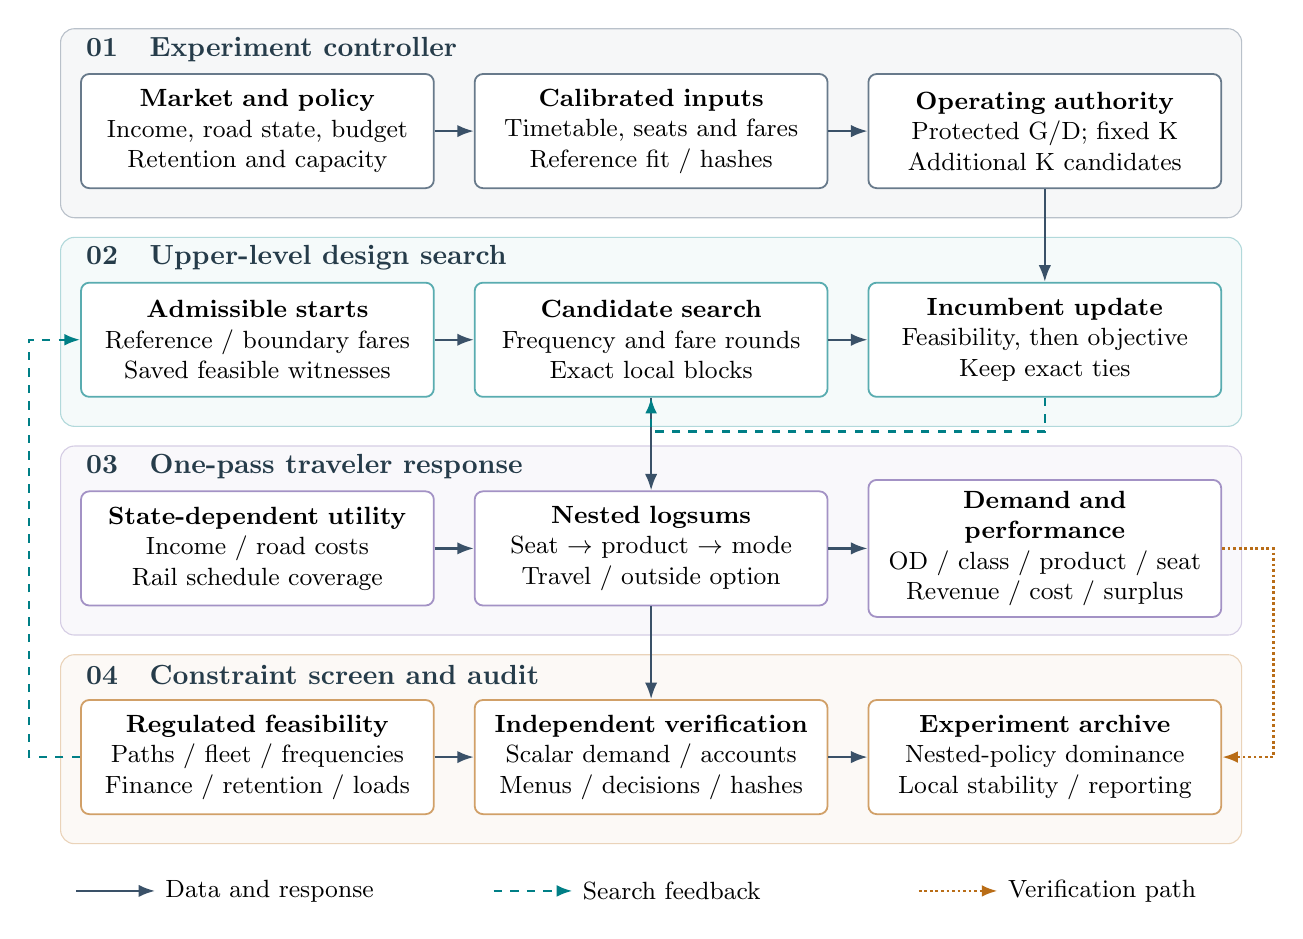
\begin{tikzpicture}[font=\fontsize{9}{11}\selectfont,
 block/.style={draw=#1!65,fill=white,rounded corners=3pt,text width=4.2cm,minimum height=1.45cm,align=center,line width=.65pt,inner sep=4pt},
 data/.style={-{Latex[length=2.1mm]},draw=navy!85,line width=.8pt},
 feedback/.style={-{Latex[length=2mm]},draw=teal,dashed,line width=.9pt},
 audit/.style={-{Latex[length=2mm]},draw=amber,densely dotted,line width=1pt}]
\foreach \y/\col/\num/\title in {0/navy/01/Experiment controller,-2.65/teal/02/Upper-level design search,-5.30/violet/03/One-pass traveler response,-7.95/amber/04/Constraint screen and audit}{
 \begin{scope}[on background layer]
 \filldraw[fill=\col!4,draw=\col!30,rounded corners=5pt] (-2.5,\y+1.30) rectangle (12.5,\y-1.10);
 \end{scope}
 \node[anchor=west,text=ink,font=\fontsize{10}{12}\selectfont\bfseries] at (-2.3,\y+1.04) {\num\quad\title};
}
\node[block=navy] (a1) at (0,0) {\textbf{Market and policy}\\Income, road state, budget\\Retention and capacity};
\node[block=navy] (a2) at (5,0) {\textbf{Calibrated inputs}\\Timetable, seats and fares\\Reference fit / hashes};
\node[block=navy] (a3) at (10,0) {\textbf{Operating authority}\\Protected G/D; fixed K\\Additional K candidates};
\node[block=teal] (b1) at (0,-2.65) {\textbf{Admissible starts}\\Reference / boundary fares\\Saved feasible witnesses};
\node[block=teal] (b2) at (5,-2.65) {\textbf{Candidate search}\\Frequency and fare rounds\\Exact local blocks};
\node[block=teal] (b3) at (10,-2.65) {\textbf{Incumbent update}\\Feasibility, then objective\\Keep exact ties};
\node[block=violet] (c1) at (0,-5.30) {\textbf{State-dependent utility}\\Income / road costs\\Rail schedule coverage};
\node[block=violet] (c2) at (5,-5.30) {\textbf{Nested logsums}\\Seat $\to$ product $\to$ mode\\Travel / outside option};
\node[block=violet] (c3) at (10,-5.30) {\textbf{Demand and performance}\\OD / class / product / seat\\Revenue / cost / surplus};
\node[block=amber] (d1) at (0,-7.95) {\textbf{Regulated feasibility}\\Paths / fleet / frequencies\\Finance / retention / loads};
\node[block=amber] (d2) at (5,-7.95) {\textbf{Independent verification}\\Scalar demand / accounts\\Menus / decisions / hashes};
\node[block=amber] (d3) at (10,-7.95) {\textbf{Experiment archive}\\Nested-policy dominance\\Local stability / reporting};
\foreach \r in {a,b,c,d}{\draw[data] (\r1.east)--(\r2.west);\draw[data] (\r2.east)--(\r3.west);}
\draw[data] (a3.south)--(b3.north);
\draw[data] (b2.south)--(c2.north);
\draw[data] (c2.south)--(d2.north);
\draw[feedback] (d1.west)--++(-.65,0)|-(b1.west);
\draw[audit] (c3.east)--++(.65,0)|-(d3.east);
\draw[feedback] (b3.south)--++(0,-.43)-|(b2.south);
\draw[data] (-2.3,-9.65)--(-1.3,-9.65) node[right,font=\small] {Data and response};
\draw[feedback] (3.0,-9.65)--(4.0,-9.65) node[right,font=\small] {Search feedback};
\draw[audit] (8.4,-9.65)--(9.4,-9.65) node[right,font=\small] {Verification path};
\end{tikzpicture}
\end{document}
